\documentclass[a4paper,titlepage]{article}
\usepackage{hyperref}
\usepackage{graphicx}
\usepackage{dingbat}
\usepackage{fancyhdr}
\usepackage{geometry}
\geometry{left=3.0truecm,right=3.0truecm,top=3.0truecm,bottom=3.0truecm} 

\author{David Acreman}
\title{Profiling for the APinTA-PDEs project}

\begin{document}
\pagestyle{fancy}
\lhead{}
\chead{}
\rhead{Profiling report}

\maketitle
\pagebreak
\tableofcontents
\pagebreak

\section{Introduction}

This document gives an overview of the profiling tools available to the APinTA-PDEs project. Although this report primarily focusses on Firedrake the profiling tools evaluated could be used for profiling other codes used by the project. Section~\ref{section:target_platforms} presents the target platforms being considered in this report and reviews the hardware and software available on these systems. 

\section{Target platforms}
\label{section:target_platforms}

The target HPC platforms for the project are Archer-2 (national tier-1), Isambard (national tier-2) and Isca (local tier-3). Isambard has two separate systems based on the ARM64 architecture: the XCI system which is an established production system, and the A64FX system which is a newer system. The A64FX system should be considered a stretch objective as the hardware and software are less well known to us. We have also purchased a local server which is designed to be similar to an Archer compute node, although it will run Ubuntu which will make it easier to build Firedrake. The server can function as a reference installation as it will use an unmodified Firedrake install script, rather than the more customised installations on the HPC platforms which will use non-standard components, for example MPI libraries and maths libraries. An overview of the hardware in the target platforms is shown in Table~\ref{tab:hardware}.
%
\begin{table}[htp]
\begin{center}
\begin{tabular}{|l|l|r|r|l|}
\hline 
System         & Processor        & Cores/node & Memory/node     & Interconnect \\
\hline
Archer-2       & AMD x86\_64         & 128        & 256 GB DRAM  & HPE Cray Slingshot  \\
Isambard XCI   & Thunder X2 ARM64    &  64        & 256 GB DRAM  & Cray Aries          \\
Isambard A64FX & Fujitsu A64FX ARM64 & 48         & 32 GB HBM    & Mellanox Infiniband \\
Isca           & Intel x86\_64       & 16/20      & 128 GB DRAM  & Mellanox Infiniband \\
Server         & AMD x86\_64         & 128        & 256 GB DRAM  & None                \\
\hline
\end{tabular}
\end{center}
\caption{Target platform hardware specifications. The Isambard A64FX platform has high bandwidth memory (HBM) which should give better performance than DRAM but has a smaller capacity.}
\label{tab:hardware}
\end{table}%

An overview of the software stacks on the target platforms is shown in Table~\ref{tab:software}. 
Each HPC platform has the GNU compilers, a compiler from the processor vendor (AMD, Intel, ARM and Fujitsu) and Cray systems also have the Cray compiler\footnote{On Isambard A64FX run \texttt{module use /lustre/software/aarch64/modulefiles} to make extra modules available}.
\begin{table}[htp]
\begin{center}
\begin{tabular}{|l|l|l|l|l|}
\hline 
System         & Compilers               & MPI libraries  & Maths lib.       & Profilers  \\
\hline
Archer-2       & Cray, GNU, AOCC         & Cray MPICH2     & Cray libsci     & Cray      \\
Isambard XCI   & Cray, GNU, ARM          & Cray MPICH2     & Cray libsci     & Cray, ARM \\
Isambard A64FX & Cray, GNU, ARM, Fujitsu & Cray MVAPICH2   & Cray libsci     & ARM       \\
Isca           & GNU                     & OpenMPI         & OpenBLAS        & None      \\
Isca           & Intel                   & Intel           & Intel MKL       & Intel     \\
Server         & GNU                     & MPICH?          & ???             & None      \\
\hline
\end{tabular}
\end{center}
\caption{Software stacks on target platforms. AOCC is the AMD Optimizing Compiler Collection. Intel MPI and MVAPICH are MPICH derivatives which support an Infiniband interconnect.
The Cray profiler is Cray Performance Analysis Tools (PAT), the ARM profilers are part of the ARM Forge tool suite and the Intel profilers are part of the Intel Parallel Studio suite.
The A64FX system did not appear to have a perftools module.}
\label{tab:software}
\end{table}
The GNU compilers are the one compiler family which is available on all the target platforms.

On the Cray systems compilation is handled by wrapper scripts from the Cray Programming Environment. The wrapper script can run different compilers depending on which programming environment module is loaded at compile time (e.g. \texttt{PrgEnv-cray} calls the Cray compiler and \texttt{PrgEnv-gnu} calls the GNU compiler). The MPI library and maths library are then linked by the wrapper script. On Cray systems the standard profiling tool is Cray Performance Analysis Tools (PAT) and on Isambard there is also the ARM Forge profiler\footnote{ARM Forge was previously known as Allinea Forge}.

The software environment on Isca is managed using Easybuild which has the concept of a toolchain. There are two toolchains on Isca: the GCC-foss toolchain and the Intel toolchain. Each toolchain has a different MPI library and maths library. Intel Parallel Studio has an MPI profiling tool called Intel Trace Analyzer and Collector (ITAC) which needs to use Intel MPI.

The server does not currently have any profiling software but an evaluation licence for ARM Forge and/or Intel Parallel Studio could be used to evaluate these tools on the server. There is also the option of installing open source profiling tools on the server. \\

\noindent
\textbf{Recommendation: standardise on the GNU compilers for all platforms. This avoids having to manage too many different builds and takes the compiler out of the performance equation (different GCC versions notwithstanding).}

%%%%%%%%%%%%%%%%%%%%%%%%%%%%%%%%%%%%%%%%%%%%%%%%%%%%%%%%%%%%%%%%%%%%%%%%%%%%%%%%%%%%%%%%%%%%%%%%%%%%%%%%%%%%%%%%%%%%%%%%%%%%%%%%%%%%%%

\section{Profiling tools}

Within Firedrake there are two ways to obtain profiling information:
\begin{itemize}
\item Add a PyOP2 timed stage
\item Request profiling information from PETSc
\end{itemize}
These options will be available on all platforms when Firedrake is the target application.

There are also external profilers which are already installed on the target platforms. Different platforms have different profilers available:
\begin{itemize}
\item ARM Forge (currently only licensed on Isambard)
\item Cray PAT (Cray systems only)
\item Intel Parallel Studio (Intel MPI only)
\end{itemize}

\subsection{Test cases}

Plan for testing external profilers:
\begin{enumerate}
\item Test with the Mandelbrot examples
\item Test with Firedrake if possible
\end{enumerate}

Use the Mandelbrot examples to show whether the profiler can spot load imbalance vs. overhead (version 1 vs. version 2) and can show the difference between collectives and point-to-point communication (version 2 vs version 3).

%---------------------------------------------------------------------------------------------------------------------

\subsection{ARM Forge}

The ARM Forge suite of development tools is available on the Isambard system. ARM Forge includes two performance tools: ``Performance Reports'' and ``MAP''. 
ARM MAP is a profiler which is part of the ARM Forge suite and it can profile C++, C, Fortran and Python\footnote{\url{https://www.arm.com/products/development-tools/server-and-hpc/forge/map}}.

%---

\subsubsection{Performance Reports}

The documentation for Performance Reports says that on Cray systems dynamic linking or explicit linking with the profiling libraries is required\footnote{\url{https://developer.arm.com/documentation/101136/2102/Performance-Reports/Get-started-with-Performance-Reports/Compile-on-Cray-X-series-systems}}. However in the latest Cray compilers dynamic linking is the default so no changes are required to the build process. The following shows an example session and output from Performance Reports on the Isambard XCI system.

No changes are required at compile time so simply compile the executable as normal. For this example the GCC compiler will be used:
\begin{verbatim}
> module switch PrgEnv-cray PrgEnv-gnu
> cc -o mandelbrot mandelbrot_mpi.c
\end{verbatim}
Two changes are required in the job script in order to activate performance reports. The first change is to load the \texttt{arm-forge} module:
\begin{verbatim}
module load tools/arm-forge
\end{verbatim}
and the second change is to add the \texttt{perf-report} command before the \texttt{aprun} command:
\begin{verbatim}
perf-report aprun -n ${nprocs} ./mandelbrot
\end{verbatim}
This method of launching a job under perf-report is referred to as Express Launch mode.
%
When the job runs two extra files are generated which contain the output from the performance report in text and HTML formats. The output from running a performance report on the Mandelbrot version 1 example using 4 MPI processes is shown in figure~\ref{fig:perf-report_MB1}.  
%
\begin{figure}[htbp]
\begin{center}
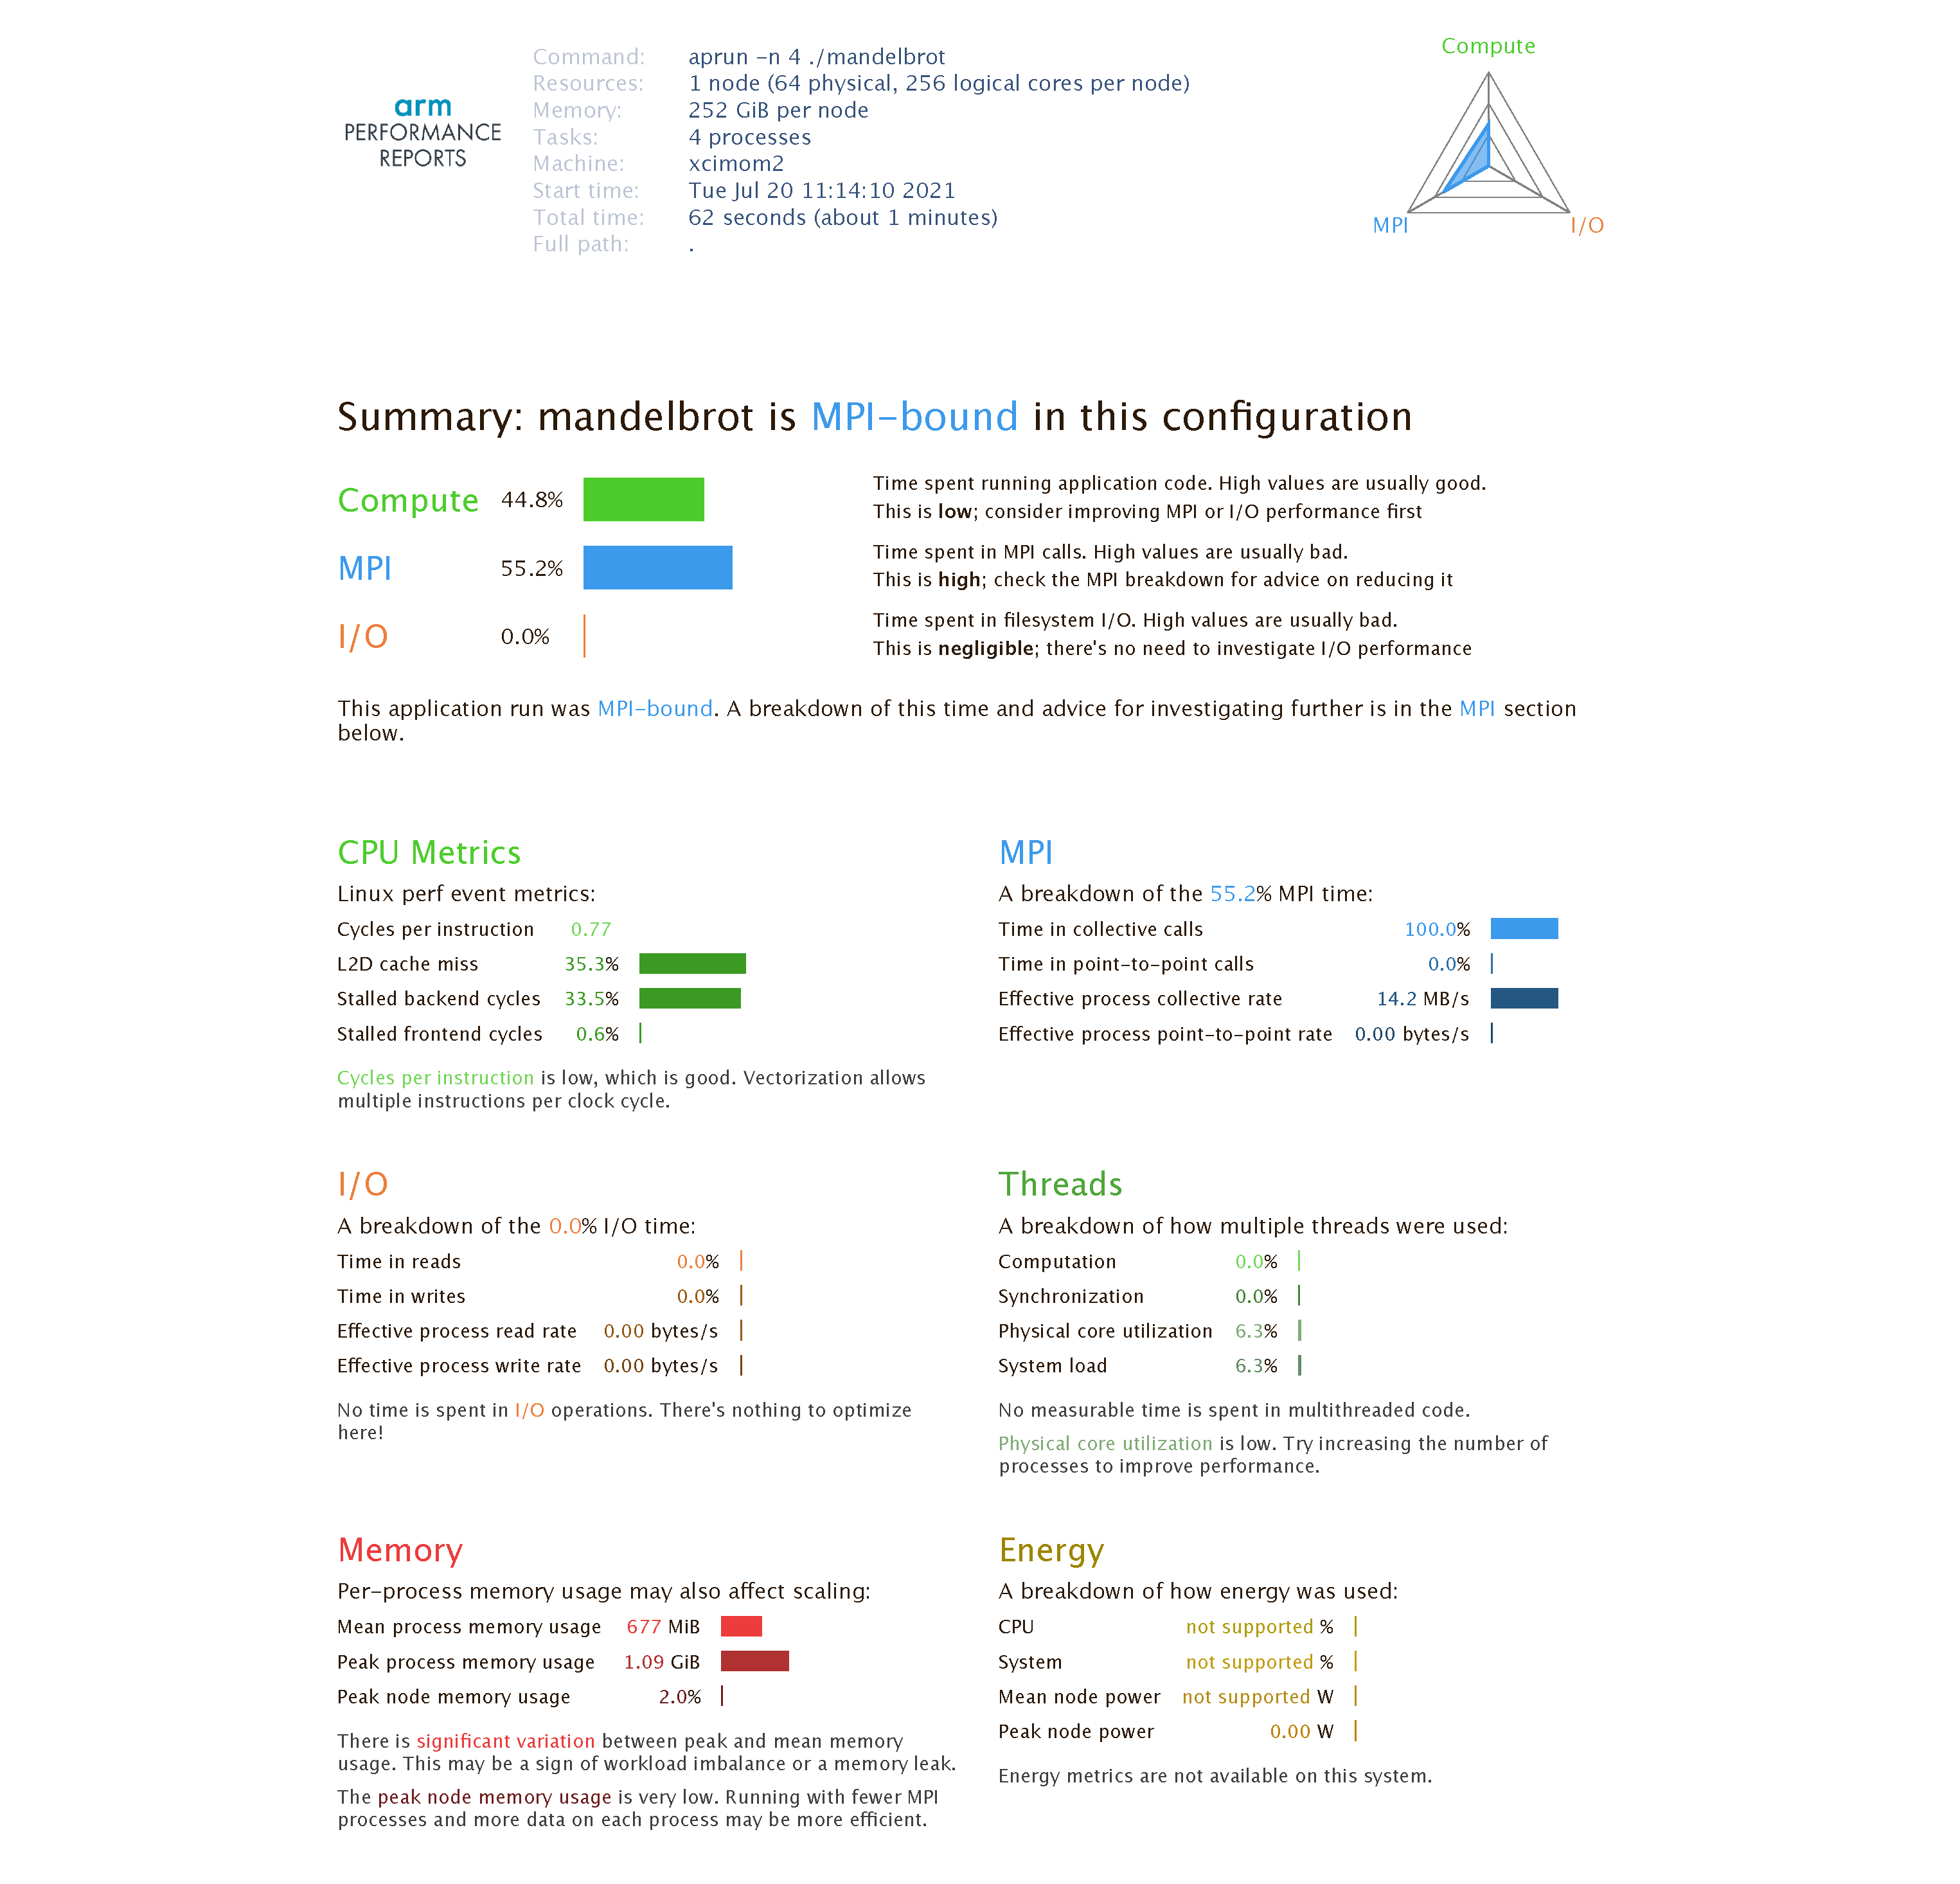
\includegraphics[scale=0.35]{figures/mandelbrot_v1_PerformanceReport}
\caption{ARM Performance Report from the Mandelbrot version 1 example. The tool correctly identifies that there is excessive time spent in MPI calls but does not identify load imbalance as the performance issue.}
\label{fig:perf-report_MB1}
\end{center}
\end{figure}
In this example the I/O has been switched off to highlight the performance issue caused by the load imbalance. The tool correctly identifies that there is excessive time spent in MPI calls but does not identify load imbalance as the performance issue. 

For the next test the I/O was switched on and the results are shown in figure~\ref{fig:perf-report_MB1_IO}.
\begin{figure}[htbp]
\begin{center}
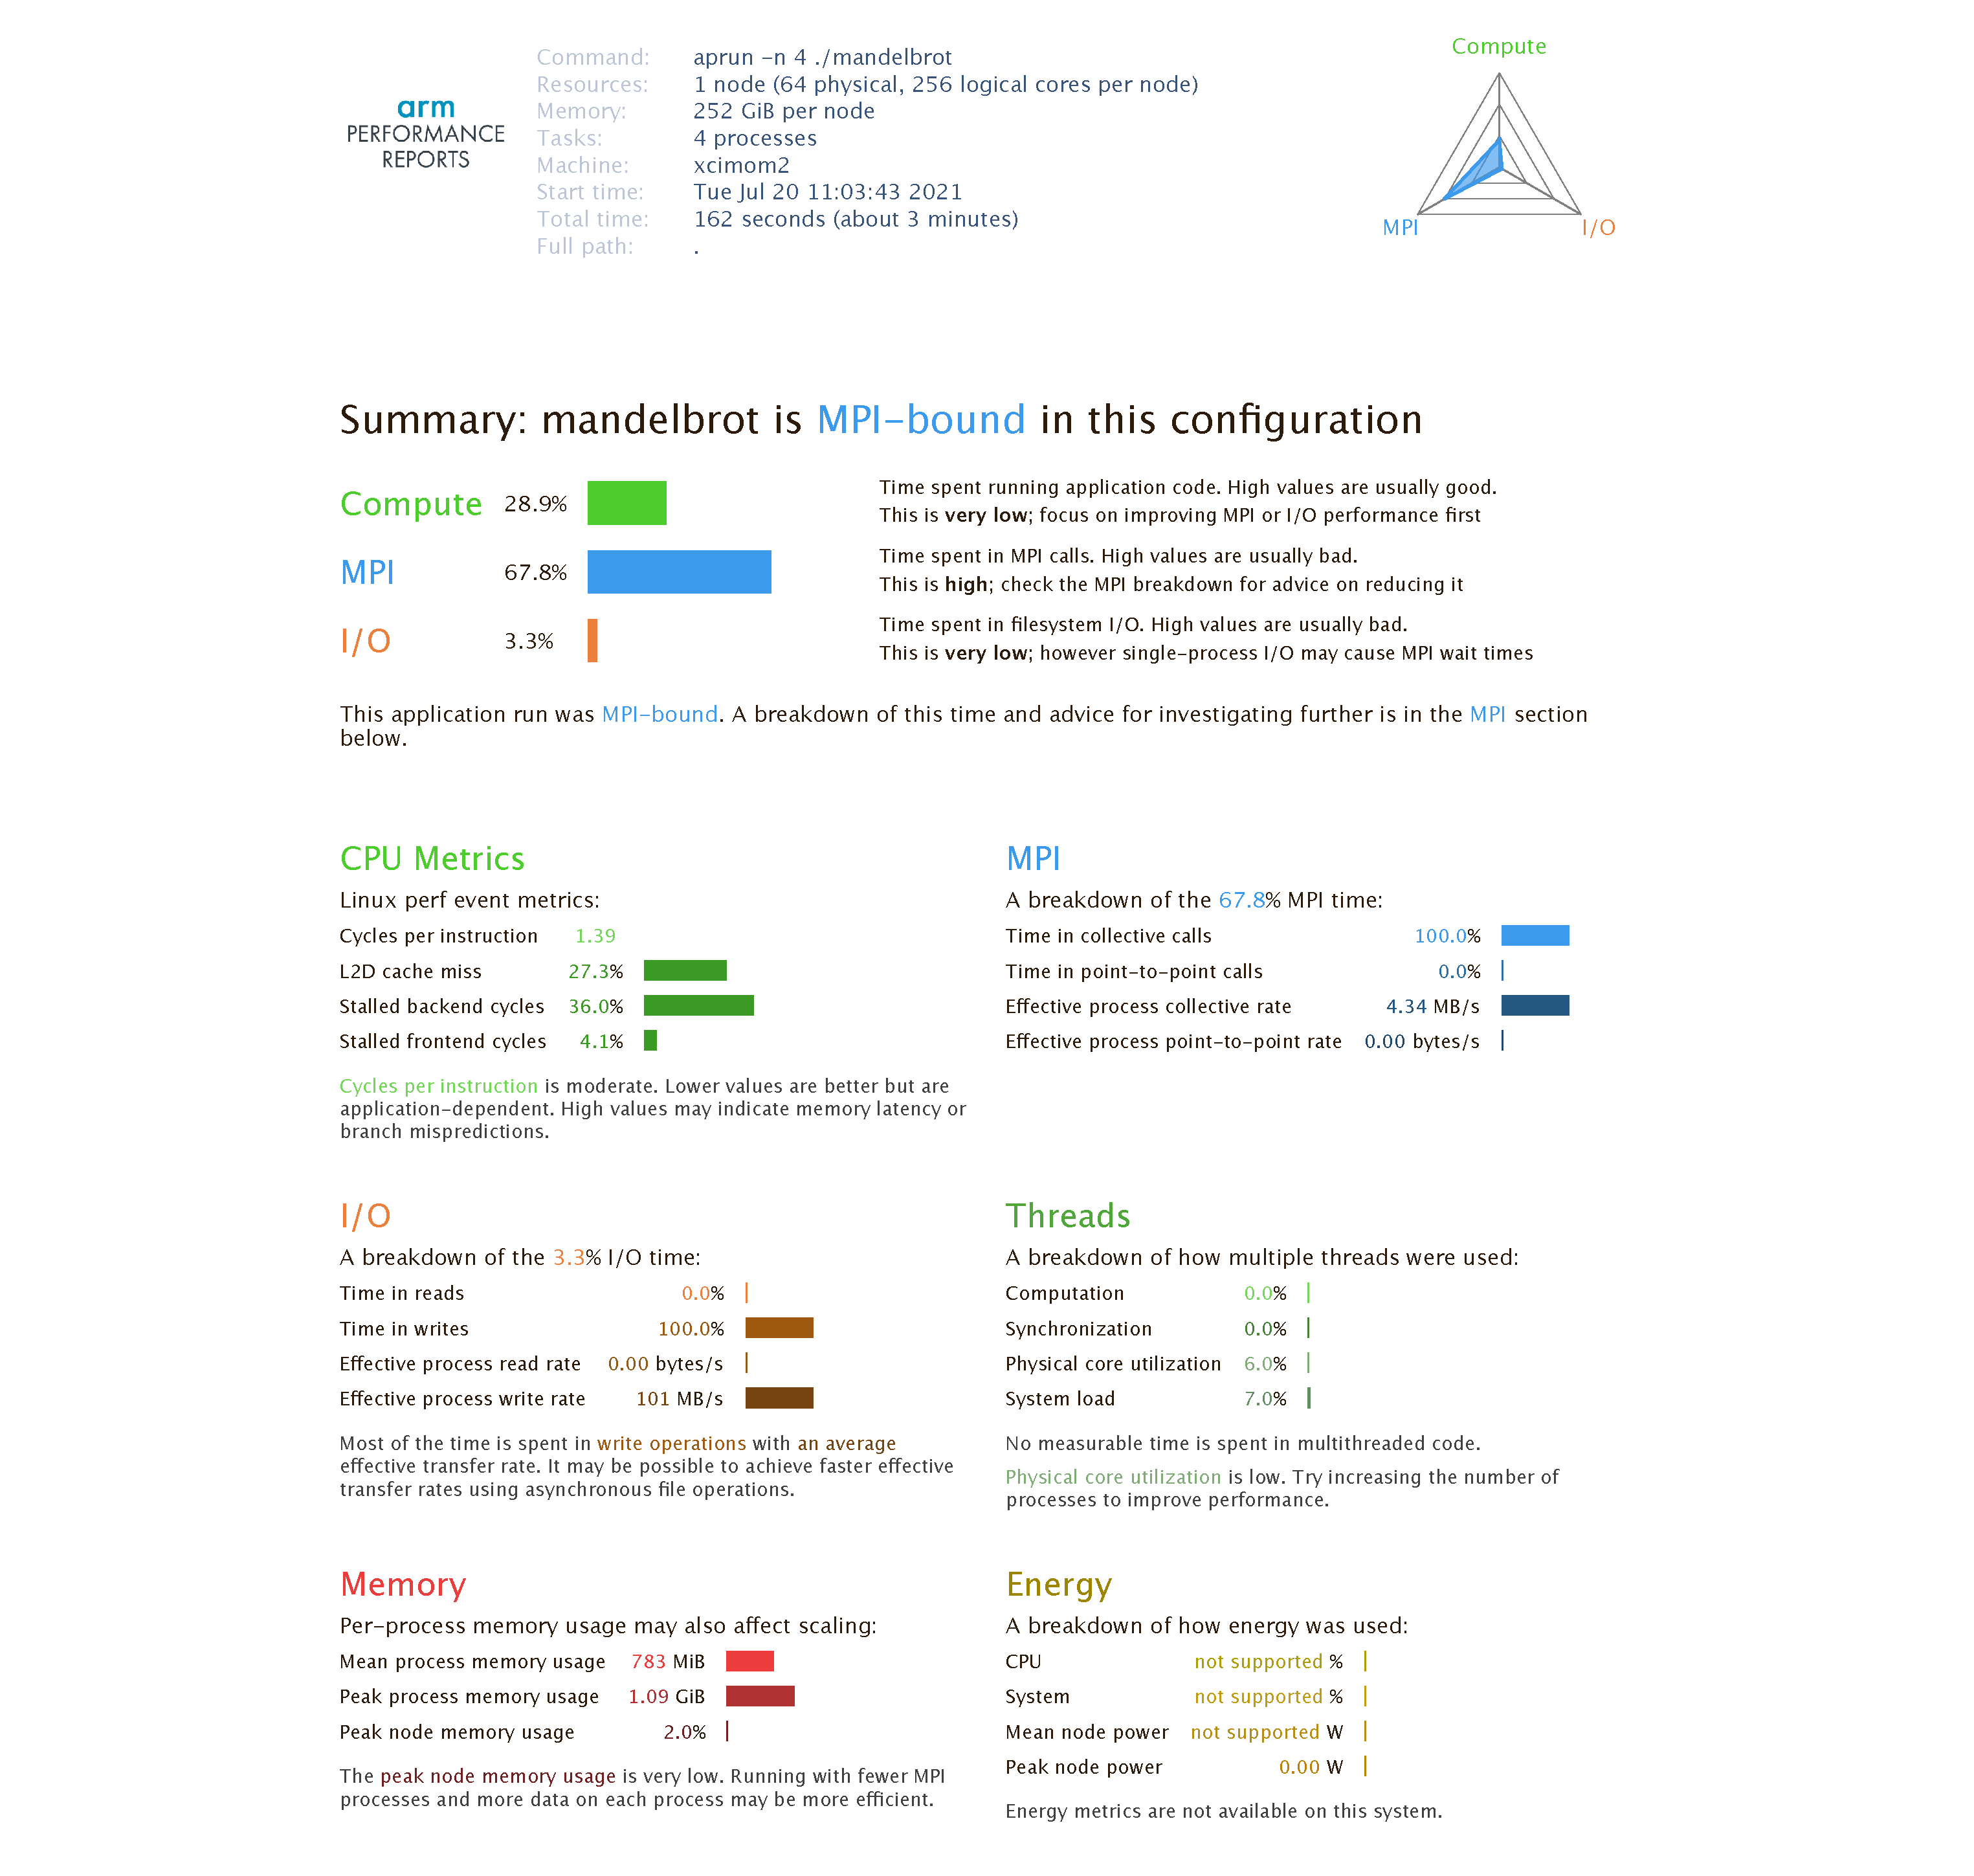
\includegraphics[scale=0.35]{figures/mandelbrot_v1_IO_PerformanceReport}
\caption{ARM Performance Report from the Mandelbrot version 1 example with I/O switched on. The additional time spent in I/O shows up as an exacerbated load imbalance due to I/O being funnelled through the rank zero process.}
\label{fig:perf-report_MB1_IO}
\end{center}
\end{figure}
The additional time spent in I/O shows up as an exacerbated load imbalance due to I/O being funnelled through the rank zero process which causes all other processes to wait at an MPI barrier. Although slow I/O is the underlying cause the time spent in I/O is only a small fraction of the time breakdown.


\begin{figure}[htbp]
\begin{center}
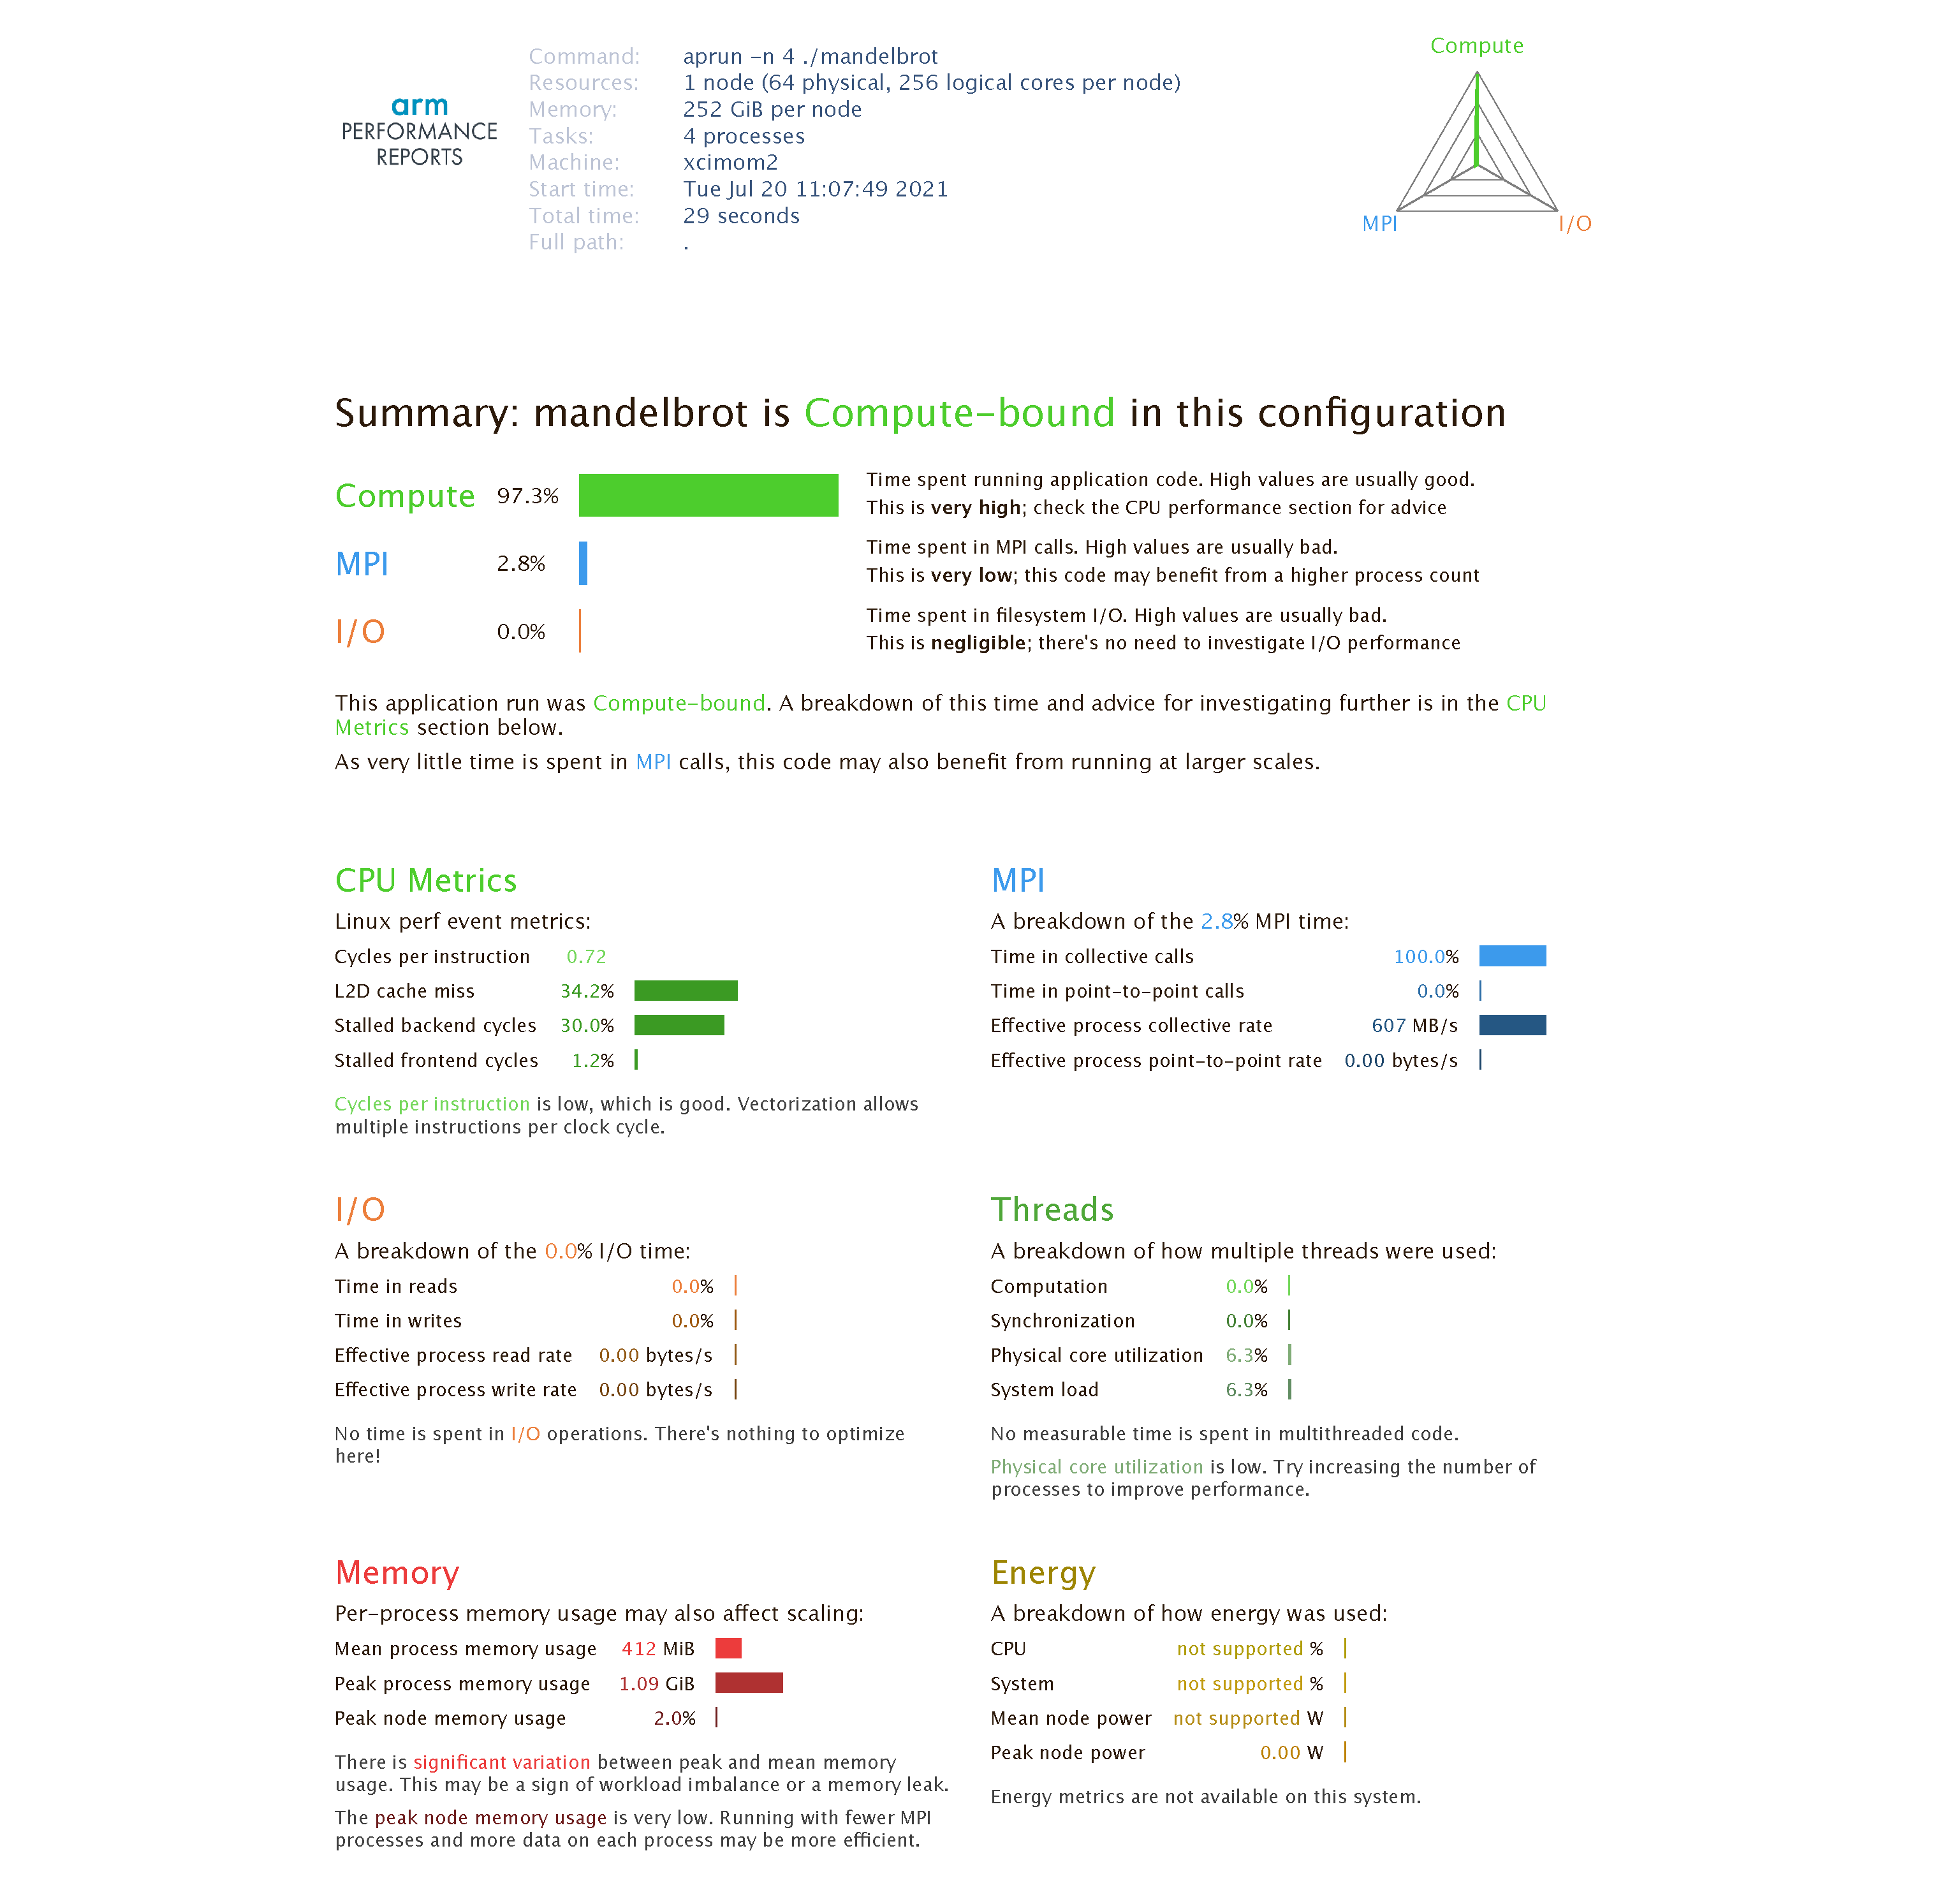
\includegraphics[scale=0.35]{figures/mandelbrot_v2_PerformanceReport}
\caption{ARM Performance Report from the Mandelbrot version 2 example. This version has fixed the load imbalance by interleaving iterations on the real axis.}
\label{fig:perf-report_MB2}
\end{center}
\end{figure}

Figure~\ref{fig:perf-report_MB3} shows the Performance Report from the Mandelbrot version 3 example with 4 MPI processes. This version of the program uses a manager-worker pattern which means that only 3 out of 4 MPI processes carry out the calculation and the fourth process is the manager which does not compute any points. The MPI time of 25\% is consistent with the manager process waiting for results from the worker processes. 
\begin{figure}[htbp]
\begin{center}
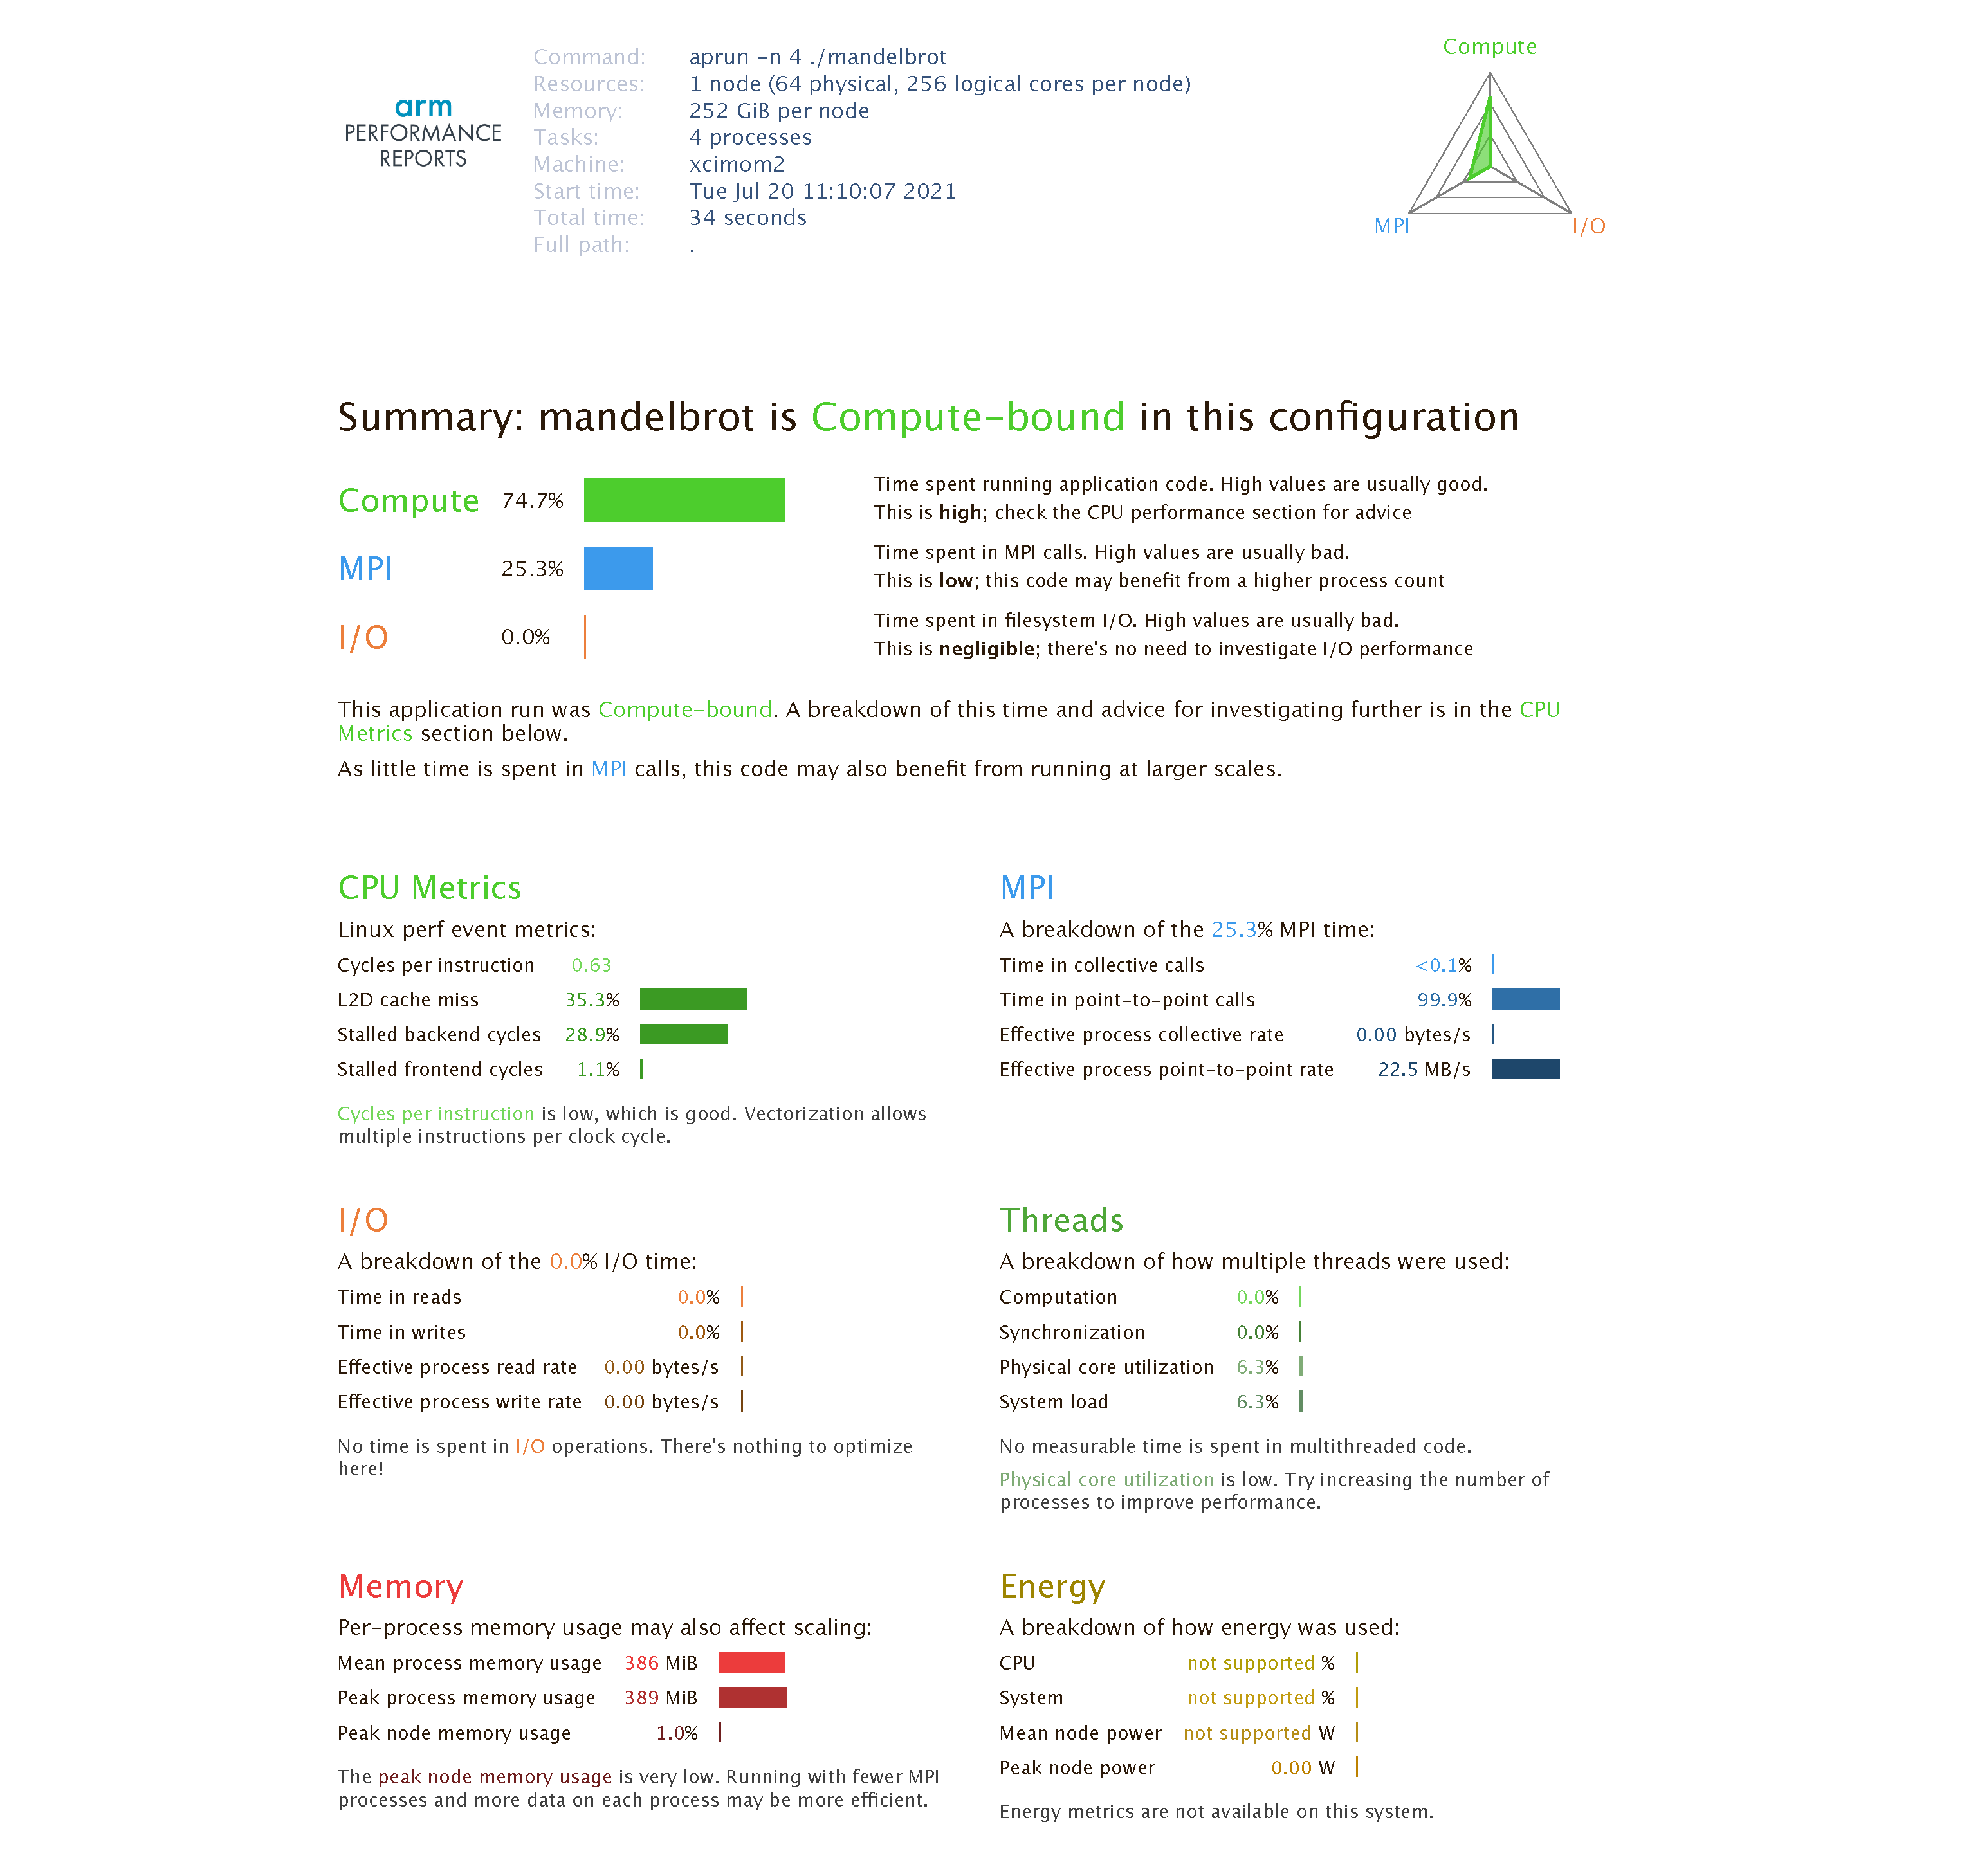
\includegraphics[scale=0.35]{figures/mandelbrot_v3_PerformanceReport}
\caption{ARM Performance Report from the Mandelbrot version 3 example with 4 MPI processes. In the manager-worker pattern only 3 out of 4 MPI processes carry out the calculation and the fourth process is the manager which does not compute any points.}
\label{fig:perf-report_MB3}
\end{center}
\end{figure}
If the number of MPI processes is increases to 16 (see figure~\ref{fig:perf-report_MB3_16procs}) then the fraction of MPI time decreases as there are now 15 processes actively working on the calculation.
\begin{figure}[htbp]
\begin{center}
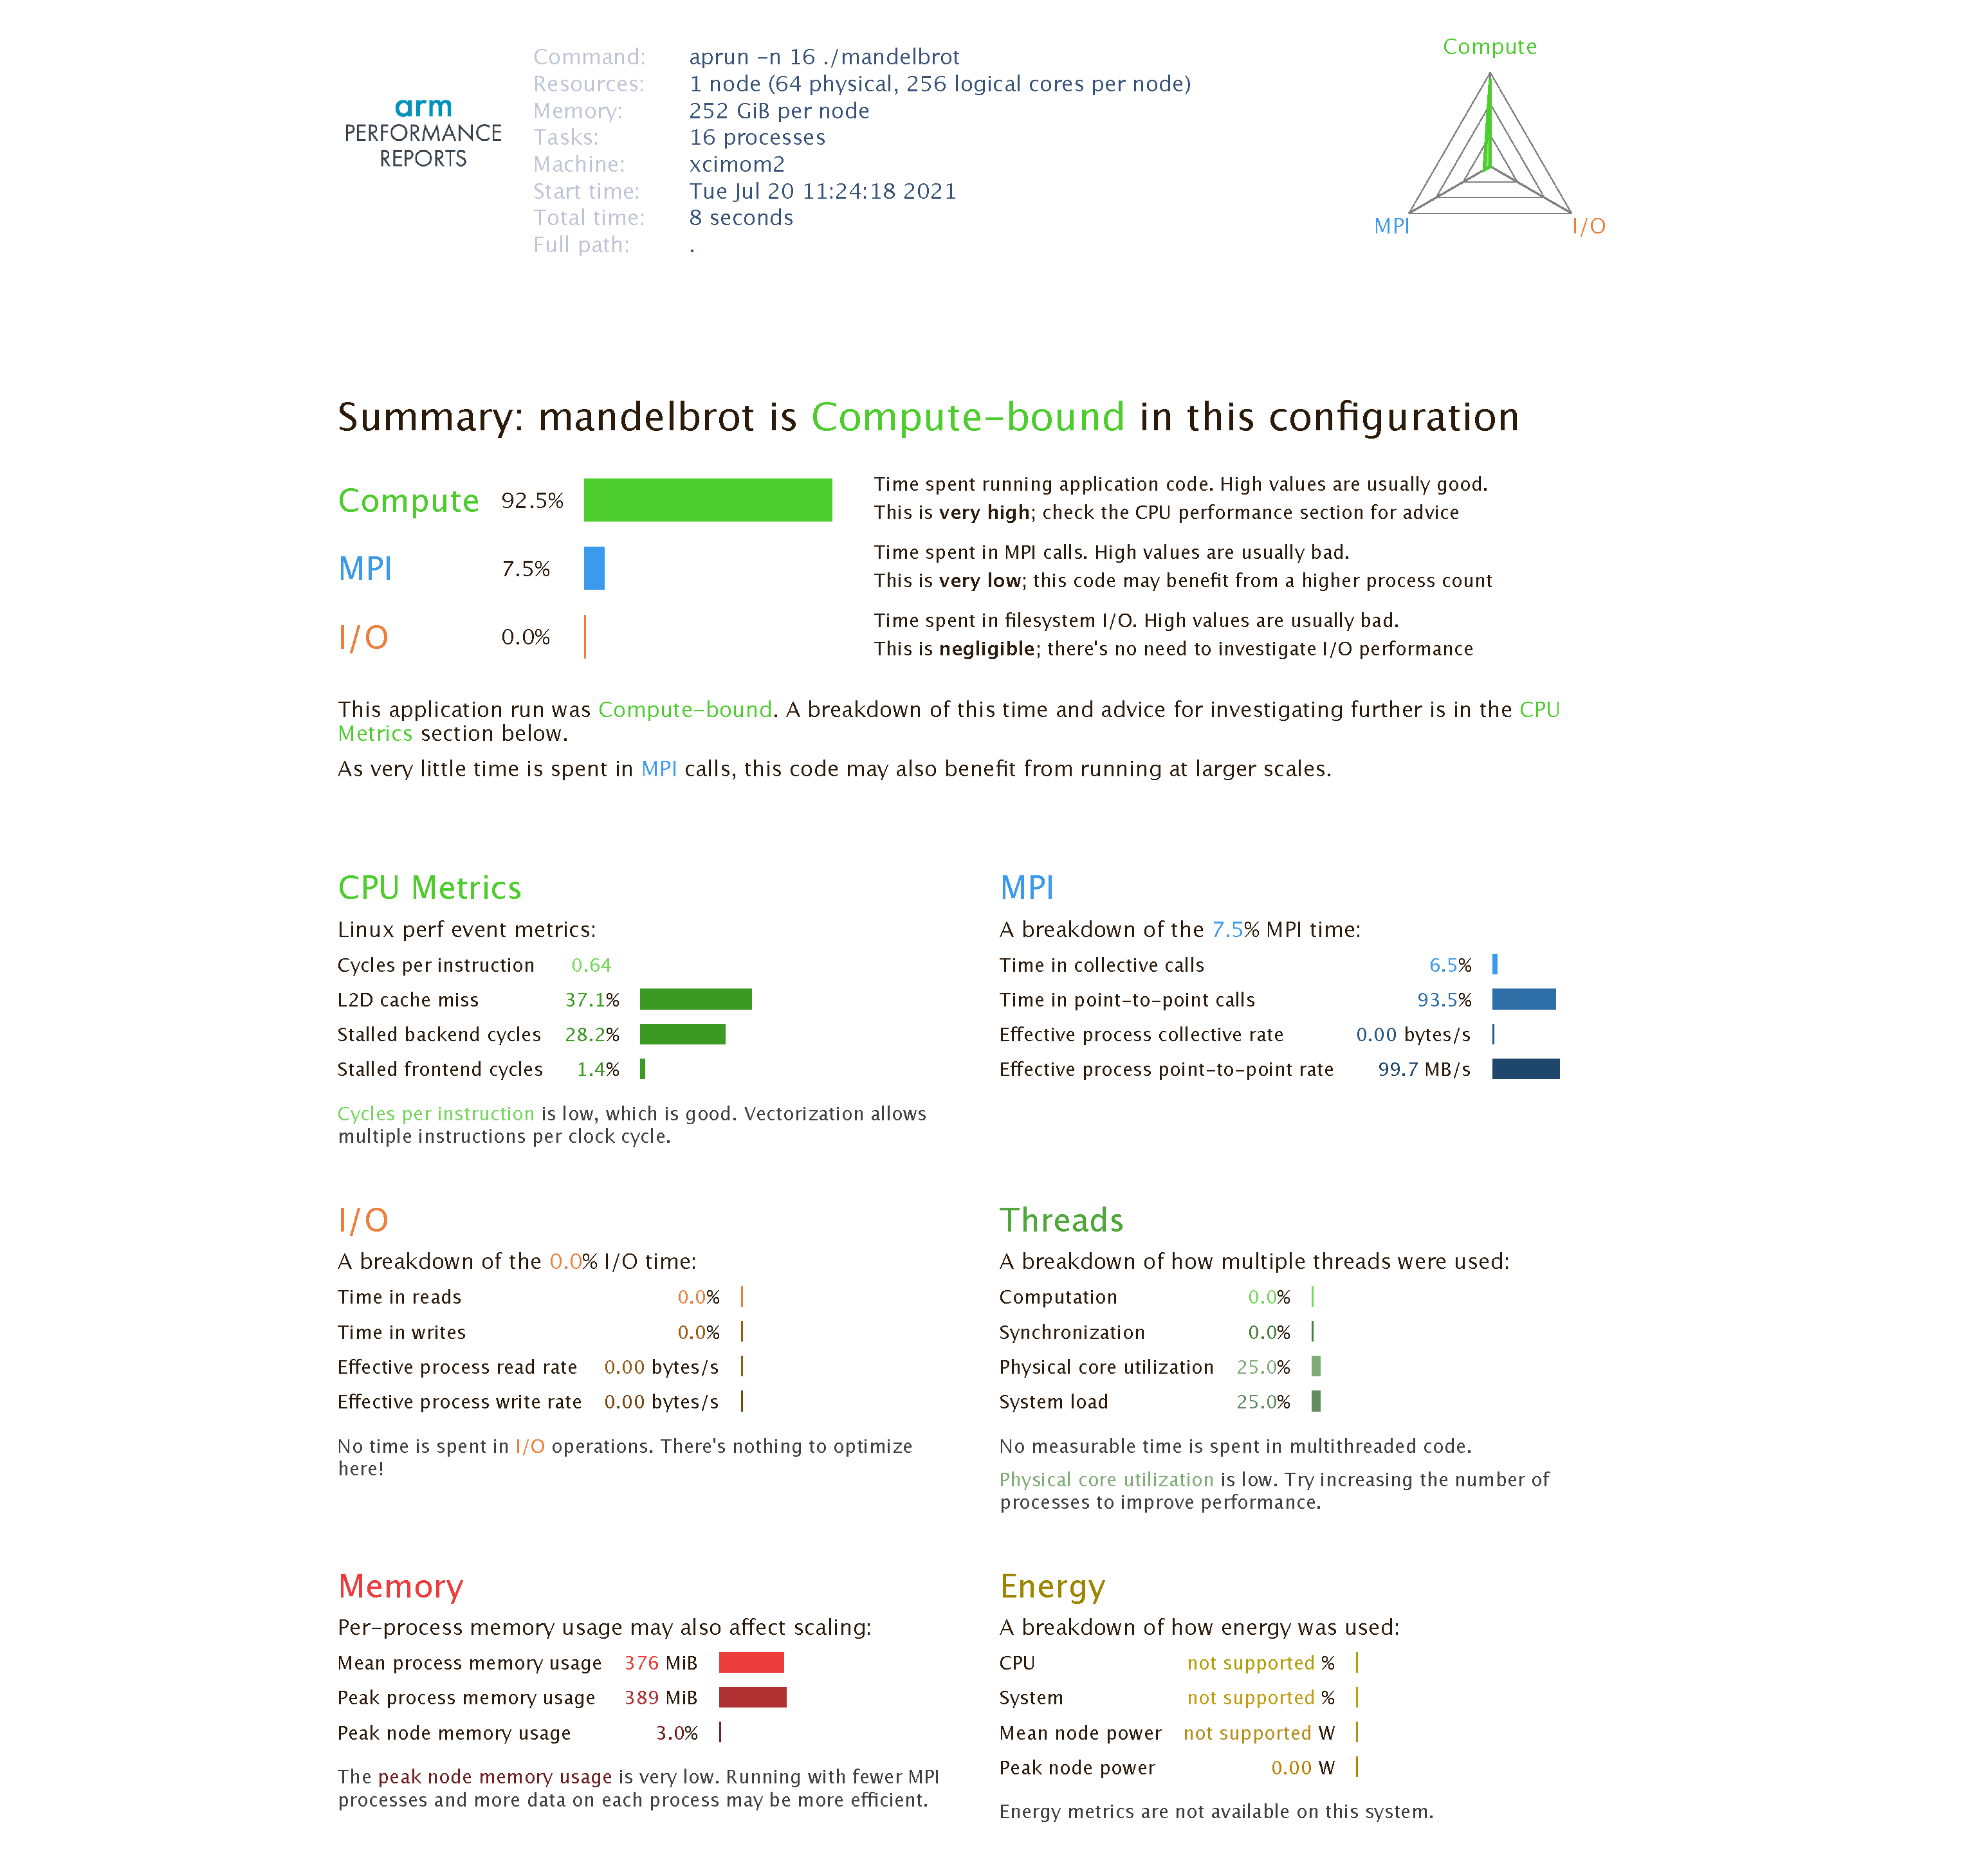
\includegraphics[scale=0.35]{figures/mandelbrot_v3_16procs_PerformanceReport}
\caption{ARM Performance Report from the Mandelbrot version 3 example with 16 MPI processes. The MPI fraction is now reduced as the manager process is only one out of 16 processes.}
\label{fig:perf-report_MB3_16procs}
\end{center}
\end{figure}

The Performance Report tool has provided a clear overview of the application performance, which highlighted the presence of performance issues, without needing to change the build process. However was not able to distinguish between load imbalance and overhead which would be clearer when viewing a time line.

%---

\subsubsection{MAP}

\subsubsection{Python}

ARM Forge can be used to profile python applications. 
Make sure to add the \verb+-j 1+ flag when using ARM profilers on Isambard otherwise there can be a hang on exit\footnote{\url{https://developer.arm.com/documentation/101136/2102/Appendix/Known-issues/Arm-MAP}} (this appears to be specific to the ARM64 architecture).

%---------------------------------------------------------------------------------------------------------------------

\subsection{Intel Parallel Studio}

Previously working on Isca with the Intel build. Intel MPI is required for the Trace Analyzer and Collector profiler to work. We should be able to use Intel MPI with the GCC compilers.

%---------------------------------------------------------------------------------------------------------------------

\subsection{Cray PAT}

Although this is a Cray tool it does work with compilers other than Cray (the other PrgEnv modules load perftools-base). Experience building SWIFT showed that the \texttt{perftools-lite} module can confuse autogen and configure so only load the module prior to the make command. 

\begin{itemize}
\item Cray PAT has two modes: standard and ``lite''
\item There is a graphical viewer (Apprentice 2) which reads the profiling output
\item Can view a time line from a full trace
\end{itemize}
See also \url{https://docs.nersc.gov/tools/performance/craypat/}.

It's not clear how to use Cray PAT with python/Firedrake. Loading the perftools-lite module and using the python from the cray-python module does not produce any profiling output.

%---------------------------------------------------------------------------------------------------------------------

\subsection{Profilers summary}

Table~\ref{tab:profiler_summary} summarises the capabilities of the profiling tools reviewed in this section.
\begin{table}[htp]
\begin{center}
\begin{tabular}{|l|c|c|c|c|}
\hline
Profiler              &  Max MPI procs  &  C/C++      & Fortran     & Python         \\
\hline
ARM Forge             &   ??            & \checkmark  &  \checkmark &  \checkmark    \\
Intel Parallel Studio &   ??            & \checkmark  &  \checkmark &  ??             \\
Cray PAT              &   Unlimited     & \checkmark  &  \checkmark &                \\
\hline
\end{tabular}
\end{center}
\caption{Summary of profiling tools}
\label{tab:profiler_summary}
\end{table}%

%%%%%%%%%%%%%%%%%%%%%%%%%%%%%%%%%%%%%%%%%%%%%%%%%%%%%%%%%%%%%%%%%%%%%%%%%%%%%%%%%%%%%%%%%%%%%%%%%%%%%%%%%%%%%%%%%%%%%%%%%%%%%%%%%%%%%%

\section{Builds}

Plan:
\begin{enumerate}
\item Working builds on main target platforms
\item Optimised builds on main target platforms: use optimised maths libraries but beware threading
\end{enumerate}
%

\begin{table}[htp]
\begin{center}
\begin{tabular}{|l|c|c|}
\hline
Platform       &  Build status   & Profilers           \\
\hline
Archer2        &  ??             & \\
Isambard XCI   &  working        & \texttt{perf-report} \\
Isambard A64FX &  ??             & \\
Isca           &  ??             & \\
Server         &  ??             & \\
\hline
\end{tabular}
\end{center}
\caption{Status of Firedrake builds and profiling for the target platforms}
\label{table:build_status}
\end{table}%

\begin{itemize}
\item Isambard build of Firedrake: what's happening with BLAS/Lapack etc? Scalapack gets built as part of the PETSc build but is also available from \texttt{libsci}
\end{itemize}


%%%%%%%%%%%%%%%%%%%%%%%%%%%%%%%%%%%%%%%%%%%%%%%%%%%%%%%%%%%%%%%%%%%%%%%%%%%%%%%%%%%%%%%%%%%%%%%%%%%%%%%%%%%%%%%%%%%%%%%%%%%%%%%%%%%%%%

\section{Conclusions and recommendations}

%%%%%%%%%%%%%%%%%%%%%%%%%%%%%%%%%%%%%%%%%%%%%%%%%%%%%%%%%%%%%%%%%%%%%%%%%%%%%%%%%%%%%%%%%%%%%%%%%%%%%%%%%%%%%%%%%%%%%%%%%%%%%%%%%%%%%%

\end{document}
